\section{Background} \label{form}
\hspace{5mm}SARS-CoV-2, also known as COVID-19, is a highly infectious respiratory disease that has significantly impacted human activity worldwide since the first case was reported in Wuhan, China, in 2019. The virus is primarily spread through respiratory droplets, making it a significant public health concern. As a result, many governments worldwide have implemented regulatory measures to control the spread of the virus. These measures include social distancing, wearing masks, and lockdowns (Haug et al., 2020). To reduce the impacts of COVID-19 on public health, not only such controls but also vaccines and cures have been developed and authorized for emergency use in many countries. Although there has been a lot of efforts to control the spread and normalize our life, the end of the pandemic is still unclear. As a result, many experts and researchers came up with the methods (i.e. Machine Learning) to predict when the pandemic will end based on the accumulated data since 2019. 

One method introduced by Younes and Hasan (2020) is to build a Generalized Lotka-Volterra (gLV) dynamic model. gLV dynamic models allow us to investigate and understand the complex interactions between populations within ecological communities. By mathematically modeling the relationships between species, these models enable us to explore how different ecological factors, such as competition and predation, impact the dynamics of populations over time. Due to the advantages that gLV has, it has been used to describe ecological interactions or phenomena.

In COVID-19 analysis using gLV (Younes and Hasan, 2020), two populations are used: (1) healthy populations and (2) infected populations. These two populations grow and diminish as they interact. For example, in the paper by Younes and Hasan (2020), they considered birth, immigration (travel), infection rate, recovery rate, death rate, and control (i.e., effectiveness of vaccines, hand washing). Following is the gLV model we will be using:
\vspace{-3mm}
\begin{center}
    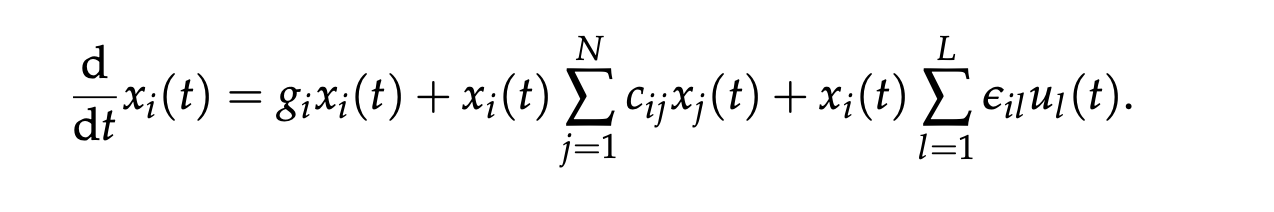
\includegraphics[width=10.5cm, 
height=1.8cm]{img/(1).png}
\end{center}
\vspace{-3mm}
The differential equations below show the population dynamics of two species considering these factors acquired by gLV above:

\vspace{5mm}
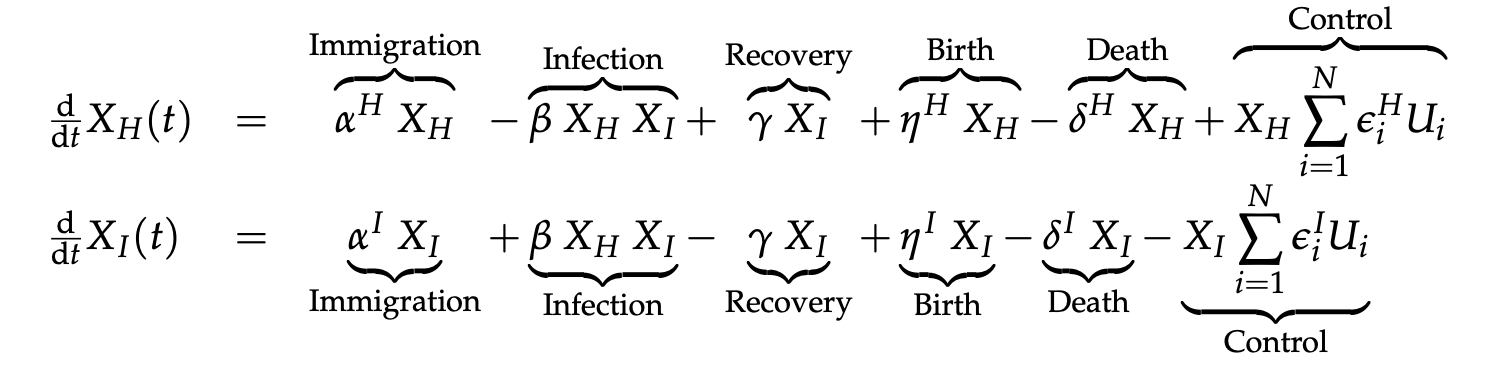
\includegraphics[width=14.5cm, height=3.7cm]{img/(2).png}
\vspace{5mm}

The variables $X_H(t)$ and $X_I(t)$ represent the healthy and infected populations over time $t$, respectively. The immigration rate, or travel rate, is denoted by $\alpha \geq 0$. If travel restrictions are imposed, $\alpha$ will be equal to 0. The infection rate is denoted by $\beta \geq 0$. In an ideal scenario where social distancing is ensured, $\beta$ will be 0. The recovery rate $\gamma$ is a fixed value of 25.5\% (the global average) in this paper. The birth and death rates are denoted by $\eta$ and $\delta$, respectively. The effectiveness of vaccines and treatments is represented by $\epsilon_H$ and $\epsilon_I$.

The control variable $u(x)$ includes border restrictions (53\%), active communication with healthcare professionals (11\%), increasing the healthcare workforce (35\%), increasing government support for vulnerable populations (41\%), and national lockdowns (25\%), as analyzed by Haug et al. (2020). 
